\documentclass[twoside,10pt]{article}
\usepackage{shlists}
\usepackage[spanish]{babel}
\usepackage[applemac]{inputenc}
\usepackage[T1]{fontenc}

\usepackage{multicol}
\usepackage{picinpar}

\usepackage{url}
\newcounter{vol}
\newcounter{num}
\newcounter{anyo}
\setcounter{vol}{7}
\setcounter{num}{2}
\setcounter{anyo}{2014}
\newcommand{\mes}{Mayo}
\usepackage{revision}


\title{\ \\ Docencia 2.0\\ \large Juan Juli\'an Merelo, Fernando 
Tricas}
\author{\LARGE Inform\'atica y `mundo real': Hackatones }


\date{}

\AutTit{Docencia 2.0}

\begin{document}
\addtocounter{page}{2}

\maketitle
\vspace*{2ex}

\begin{multicols}{2}
Mucho se habla en las ense\~{n}anzas t\'ecnicas, y en particular en la
de la inform\'atica, de enlazarlas con la realidad social y
empresarial que existe fuera de la academia.  Para lograr este enlace
tenemos el enfoque tradicional, basado en la realizaci\'{o}n de
trabajos de fin de carrera, pr\'acticas en empresas de muy diverso
tipo y el propio desarrollo de las asignaturas, que en la mayor\'{i}a
de los casos no est\'an tan alejadas de la realidad como se afirma.
Pero ya llevamos una temporada larga escuchando hablar (y
participando, en algunos casos) de nuevas formas de sumergir al
alumnado en la realidad del desarrollo de proyectos inform\'aticos.
Un hackat\'{o}n es un marat\'{o}n de programaci\'{o}n, de hack, que
estrictamente ser\'{i}a hacer una \~{n}apa o apa\~{n}o en un proyecto.
En general, se trata de llevar a cabo un proyecto de programaci\'{o}n
en un tiempo limitado.  La idea es bastante simple, pero llevarla a
cabo no es trivial; integrarla dentro de un curr\'{i}culum de
ense\~{n}anza de alguna asignatura de inform\'atica tampoco.  En
realidad, cualquier asignatura que tenga pr\'acticas no tendr\'a
demasiado complicado a\~{n}adirlo, pero para que resulte especialmente
\'{u}til hacen falta una serie de requisitos.  El primero, que
efectivamente los contenidos de la asignatura est\'en enfocados a
llevar a cabo un proyecto, que puede ser dise\~{n}ar un sistema,
programarlo o poner en marcha una empresa relacionada con el mismo.
No ser\'a tan \'{u}til en asignaturas que no incluyan esa habilidad,
por ejemplo una de contenido matem\'atico.  Segundo, que se propongan
una serie de proyectos atractivos y reales, donde los alumnos
realmente vean el fruto de su trabajo.  Tercero, que la evaluaci\'{o}n
del trabajo sea tambi\'en lo m\'as real posible.  Si los proyecto han
sido propuestos por una persona de una empresa, habr\'a que contar con
ella para evaluarlos a ver si han alcanzado los objetivos.  Hay que
hacer notar aqu\'{i} que el realismo de los proyectos puede ser tan
variable como el de la industria: desde resolver necesidades puntuales
de proyectos completos y m\'as complejos a realizar desarrollos
puramente prospectivos y exploratorios para probar las posibilidades
de determinadas tecnolog\'{i}as; el principal requisito de un proyecto
es que tenga objetivos alcanzables dentro del tiempo destinado al
hackat\'{o}n y que se pueda evaluar si se han alcanzado o no los
objetivos del mismo.  Puede haber un cliente concreto (alguien que
quiere conseguir determinada caracter\'{i}stica para alg\'{u}n
producto) o los clientes pueden ser los propios desarrolladores y su
deseo puede ser el de agradar al jurado o tribunal (si se plantea como
un concurso) o a la sociedad y personas relacionadas con la
convocatoria.  Adem\'as de la componente de desarrollo inform\'atico,
un hackat\'{o}n incluye t\'{i}picamente algunas otras de las
competencias transversales que se reclaman a la Universidad
espa\~{n}ola: formar equipos y trabajar dentro de ellos ---a veces ser
l\'{i}der, otras ser un componente m\'as; en cualquier caso,
coordinarse para llevar a cabo los objetivos propuestos---, discutir
ideas y alternativas, utilizar herramientas de coordinaci\'{o}n,
trabajar en la comunicaci\'{o}n del avance del proyecto mientras se
desarrolla, y posteriormente a los otros equipos y personas
interesadas en exposiciones m\'as o menos p\'{u}blicas.  Finalmente,
qui\'en sabe si tomar la decisi\'{o}n de llevar el proyecto a etapas
posteriores con su mantenimiento, evoluci\'{o}n y tal vez
comercializaci\'{o}n.  En todo caso, como profesores podr\'{i}amos
pensar en realizar un hackat\'{o}n sobre proyectos que consideremos
relevantes (\textquestiondown puesta al d\'{i}a de alguna
funcionalidad para nuestro centro?)  pero tambi\'en podr\'{i}amos
animar al alumnado a participar en hackatones que se organicen en el
contexto local.  En este \'{u}ltimo caso suelen aparecer algunos
resultados laterales nada despreciables: contacto con la sociedad,
mediante el conocimiento por parte de la comunidad que organiz\'{o} el
encuentro de nuestros estudiantes universitarios
\noindent\rule{86mm}{1pt}

\vspace{1ex} {\small{\begin{window}[0,r,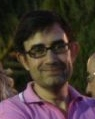
\includegraphics[width = 27
mm]{JJM.jpg},] \noindent\emph{JJ Merelo} es catedr\'{a}tico de Universidad
en el \'area de Arquitectura y Tecnolog\'{\i}a de Computadores, y
actualmente director de la Oficina de Software Libre de la UGR.
Mantiene un blog desde el a\~no 2002, y lo ha utilizado en clase desde
el a\~no 2004; tambi\'en wikis y, ultimamente, agregadores y otras
herramientas TIC. \'{U}ltimamente le ha dado por el \textsl{flipped
learning}, de lo que se informar\'{a} debidamente en esta columna.
\end{window}}}

\medskip

{\small{\begin{window}[0,r,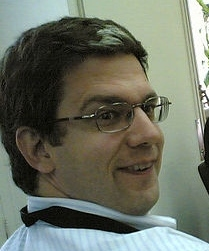
\includegraphics[width = 27 mm]{FTricas1.jpg},]
		\noindent  \emph{Fernando Tricas Garc\'{\i}a} es profesor
		titular de Lenguajes y Sistemas Inform\'aticos del Departamento
		de Inform\'atica e Ingenier\'{\i}a de Sistemas de la Universidad de
		Zaragoza.  Empez\'o a estudiar la blogosfera casi cuando a\'un no
		exist\'{\i}a (all\'a por el a\~no 2002) y a tratar de integrarla en los
		cursos y tareas docentes un poco despu\'es.  Ha impartido
		numerosas charlas relacionadas con el tema de la Web 2.0.
		Es actualmente Director de su departamento.  
		\end{window}}}

\noindent   y creaci\'{o}n de relaciones; nuestros estudiantes descubren que
pueden interaccionar con desarrolladores del 'mundo real' y sacar adelante
proyectos a su mismo nivel; tambi\'en descubren que hay aspectos que
desconocen y a los que deber\'an prestar m\'as atenci\'{o}n (t\'{i}picamente aspectos
de comunicaci\'{o}n, pero tambi\'en tecnolog\'{i}as y formas de trabajar con las que
no hab\'{i}an tenido contacto); qui\'en sabe si hasta oportunidades laborales y
de mayor implicaci\'{o}n en nuevos proyectos.
Muchas de estos resultados los vimos en el hackat\'{o}n que se hizo como \'{u}ltima
pr\'actica de la asignatura Inform\'atica Virtual del Grado en Ingenier\'{i}a
Inform\'atica en la UGR
\url{http://jj.github.io/IV/documentos/practicas/4.Aplicaciones}. El hackat\'{o}n
final se hizo conjuntamente con otra asignatura, Dise\~{n}o de Aplicaciones
para Internet y se llev\'{o} a cabo durante un fin de semana (de viernes por la
ma\~{n}ana a lunes por la ma\~{n}ana) en un espacio de coworking, de forma que el
espacio de trabajo tambi\'en fuera lo m\'as real posible. La idea original
parti\'{o} de una conferencia de Juan Freire en el que se comentaban las
experiencias en el MediaLab Prado. Todos los alumnos consideraron la
pr\'actica muy positiva o positiva
\url{https://docs.google.com/forms/d/1kzeksc0fWkReZbf3vFp5i77hoasGW8zyoP_CmYqOCdE/viewanalytics}
y, de hecho, pensamos repetirla en a\~{n}os sucesivos y quiz\'as ampliarla a
otras asignaturas.

\bigskip

\noindent\emph{Todas las columnas de la serie Docencia 2.0
pueden descargarse en formato LaTeX desde
{\small\url{https://github.com/ReVision-Docencia-20/Columnas}}}

\noindent\rule{90mm}{1pt}

{\small \noindent\copyright 2014 JJ. Merelo, F. Tricas. Este art\'{\i}culo es de acceso libre distribuido bajo los t\'erminos
de la Licencia Creative Commons de Atribuci\'on, que permite copiar,
distribuir y comunicar p\'ublicamente la obra en cualquier medio, s\'olido
o electr\'onico, siempre que se acrediten a los autores y fuentes
originales}

\end{multicols}
\end{document}
